\documentclass[aspectratio=169,10pt]{beamer}
% Shared Beamer style for MA 25-31018 Persamaan Diferensial Parsial
\usepackage[utf8]{inputenc}
\usepackage[T1]{fontenc}
\usepackage{lmodern}
\usepackage{amsmath,amssymb,mathtools,bm}
\usepackage{graphicx}
\usepackage{booktabs,array}
\usepackage{listings}
\usepackage{xcolor}
\usepackage{tikz}
\usetikzlibrary{calc,positioning,decorations.pathreplacing}

\definecolor{pdpNavy}{HTML}{0F172A}
\definecolor{pdpTeal}{HTML}{0F766E}
\definecolor{pdpMint}{HTML}{CCFBF1}
\definecolor{pdpAmber}{HTML}{F59E0B}
\definecolor{pdpSlate}{HTML}{334155}
\definecolor{pdpBg}{HTML}{F8FAFC}
\definecolor{pdpLine}{HTML}{CBD5E1}
\definecolor{pdpSoftTeal}{HTML}{ECFDF5}
\definecolor{pdpSoftAmber}{HTML}{FFF7ED}

\setbeamercolor{normal text}{fg=pdpNavy,bg=pdpBg}
\setbeamercolor{frametitle}{fg=pdpNavy,bg=pdpBg}
\setbeamercolor{title}{fg=pdpNavy}
\setbeamercolor{subtitle}{fg=pdpTeal}
\setbeamercolor{block title}{fg=white,bg=pdpTeal}
\setbeamercolor{block body}{fg=pdpNavy,bg=white}
\setbeamercolor{alerted text}{fg=pdpAmber!85!black}
\setbeamerfont{title}{series=\bfseries,size=\Large}
\setbeamerfont{frametitle}{series=\bfseries,size=\large}
\setbeamerfont{block title}{series=\bfseries}
\setbeamertemplate{navigation symbols}{}
\setbeamertemplate{itemize item}{\color{pdpTeal}$\blacktriangleright$}
\setbeamertemplate{itemize subitem}{\color{pdpAmber}$\bullet$}
\setbeamersize{text margin left=.65cm,text margin right=.65cm}

\newcommand{\pdpfooter}[2]{%
\setbeamertemplate{footline}{%
  \leavevmode\hbox{%
  \begin{beamercolorbox}[wd=.34\paperwidth,ht=2.55ex,dp=1.05ex,leftskip=.65cm]{author in head/foot}%
    \scriptsize Tim Pengajar PDP
  \end{beamercolorbox}%
  \begin{beamercolorbox}[wd=.40\paperwidth,ht=2.55ex,dp=1.05ex,center]{title in head/foot}%
    \scriptsize #1
  \end{beamercolorbox}%
  \begin{beamercolorbox}[wd=.26\paperwidth,ht=2.55ex,dp=1.05ex,rightskip=.65cm plus1fil]{date in head/foot}%
    \scriptsize Rifky Fauzi\hfill\insertframenumber/\inserttotalframenumber
  \end{beamercolorbox}}\vskip0pt% 
}}

\newcommand{\pdporangeline}{\vspace{0.15em}\textcolor{pdpAmber}{\rule{0.9cm}{1.3pt}}\vspace{0.35em}}
\newcommand{\pdpnote}[1]{{\scriptsize\color{pdpSlate}#1}}
\newcommand{\pdpkey}[1]{\textbf{\color{pdpTeal}#1}}
\newcommand{\pdpsource}[1]{{\fontsize{5.5}{6.2}\selectfont\color{pdpSlate}#1}}
\newcommand{\pdppill}[1]{\tikz[baseline=(X.base)]\node[fill=pdpMint,draw=pdpTeal,rounded corners=3pt,inner xsep=5pt,inner ysep=2pt](X){\scriptsize\bfseries #1};}

\lstdefinestyle{matlab}{
  language=Matlab,
  basicstyle=\ttfamily\scriptsize,
  keywordstyle=\color{pdpTeal}\bfseries,
  commentstyle=\color{pdpSlate},
  stringstyle=\color{pdpAmber!80!black},
  showstringspaces=false,
  breaklines=true,
  frame=single,
  framerule=0.4pt,
  rulecolor=\color{pdpLine},
  backgroundcolor=\color{white},
  xleftmargin=1mm,
  xrightmargin=1mm
}

\pdpfooter{Pertemuan 9 - Persamaan Gelombang}{}

\title{Persamaan Gelombang}
\subtitle{Pemodelan, Klasifikasi, Bentuk Kanonik, dan Solusi Analitik}
\author{Tim Pengajar Persamaan Diferensial Parsial}
\institute{Program Studi Matematika - Institut Teknologi Sumatera}
\date{Pertemuan 9 - dilaksanakan pada Minggu 10}

\begin{document}

% 1 -----------------------------------------------------------------
\begin{frame}[plain]
  \begin{tikzpicture}[remember picture,overlay]
    \fill[pdpNavy] (current page.south west) rectangle ([xshift=0.33\paperwidth]current page.north west);
    \fill[pdpTeal] ([xshift=0.33\paperwidth]current page.south west) rectangle ([xshift=0.337\paperwidth]current page.north west);
  \end{tikzpicture}
  \vspace{0.62cm}
  \begin{columns}[T]
    \column{0.30\textwidth}
      \color{white}
      {\bfseries MA 25-31018}\par\vspace{0.25cm}
      {\Large\bfseries PERSAMAAN\\ DIFERENSIAL\\ PARSIAL}\par\vspace{0.95cm}
      {\color{pdpMint}\large\bfseries Pertemuan 9}\par\vspace{0.10cm}
      {\scriptsize Dilaksanakan pada Minggu 10}
    \column{0.64\textwidth}
      {\Huge\bfseries Persamaan Gelombang}\par
      \pdporangeline
      {\Large Pemodelan, Klasifikasi, Bentuk Kanonik, dan Solusi Analitik}\par\vspace{0.62cm}
      {\bfseries Koordinator:} Dear Michiko Mutiara Noor, M.Si.\par
      {\bfseries Tim pengajar:} Dr. Dewi Suhika, M.Sc. dan Rifky Fauzi\par\vspace{0.78cm}
      Program Studi Matematika\par
      Institut Teknologi Sumatera
  \end{columns}
\end{frame}

% 2 -----------------------------------------------------------------
\begin{frame}{Agenda Pertemuan}
\begin{columns}[T,onlytextwidth]
\column{0.48\textwidth}
\begin{block}{Fondasi konseptual}
\begin{enumerate}
  \item PDP sebagai model medan ruang--waktu.
  \item Dari karakteristik orde satu ke mekanisme orde dua.
  \item Mengapa model nyata sering membutuhkan simulasi komputer.
  \item Klasifikasi: eliptik, parabolik, hiperbolik; linearitas dan kehomogenan dibedakan.
\end{enumerate}
\end{block}
\column{0.48\textwidth}
\begin{block}{Fokus matematis hari ini}
\begin{enumerate}
  \setcounter{enumi}{4}
  \item Penurunan persamaan gelombang dari vibrating string.
  \item Karakteristik dan bentuk kanonik.
  \item Solusi analitik: d'Alembert, pemisahan variabel, fungsi eigen.
  \item Linear shallow-water sebagai persamaan gelombang.
  \item Latihan individu tertulis tangan.
\end{enumerate}
\end{block}
\end{columns}
\end{frame}

% 3 -----------------------------------------------------------------
\begin{frame}{PDP sebagai Model Medan Ruang--Waktu dalam Sains Komputasi}
\begin{columns}[T,onlytextwidth]
\column{0.40\textwidth}
\footnotesize
Banyak persoalan modern tidak hanya meminta satu angka, tetapi sebuah \pdpkey{medan}: temperatur, tekanan, kecepatan, elevasi muka air, deformasi, atau konsentrasi yang berubah pada ruang dan waktu.

\vspace{0.18cm}
Pada era sensor, citra satelit, dan \emph{big data}, data menginformasikan keadaan sistem. PDP menyediakan \textbf{struktur fisis} yang menghubungkan keadaan tersebut dalam ruang dan waktu.

\vspace{0.18cm}
\begin{block}{Contoh: digital twin}
Observasi dipadukan dengan model komputasi untuk memperbarui keadaan sistem, menguji skenario, dan menghasilkan prediksi yang konsisten dengan hukum fisis.
\end{block}
\column{0.58\textwidth}
\centering
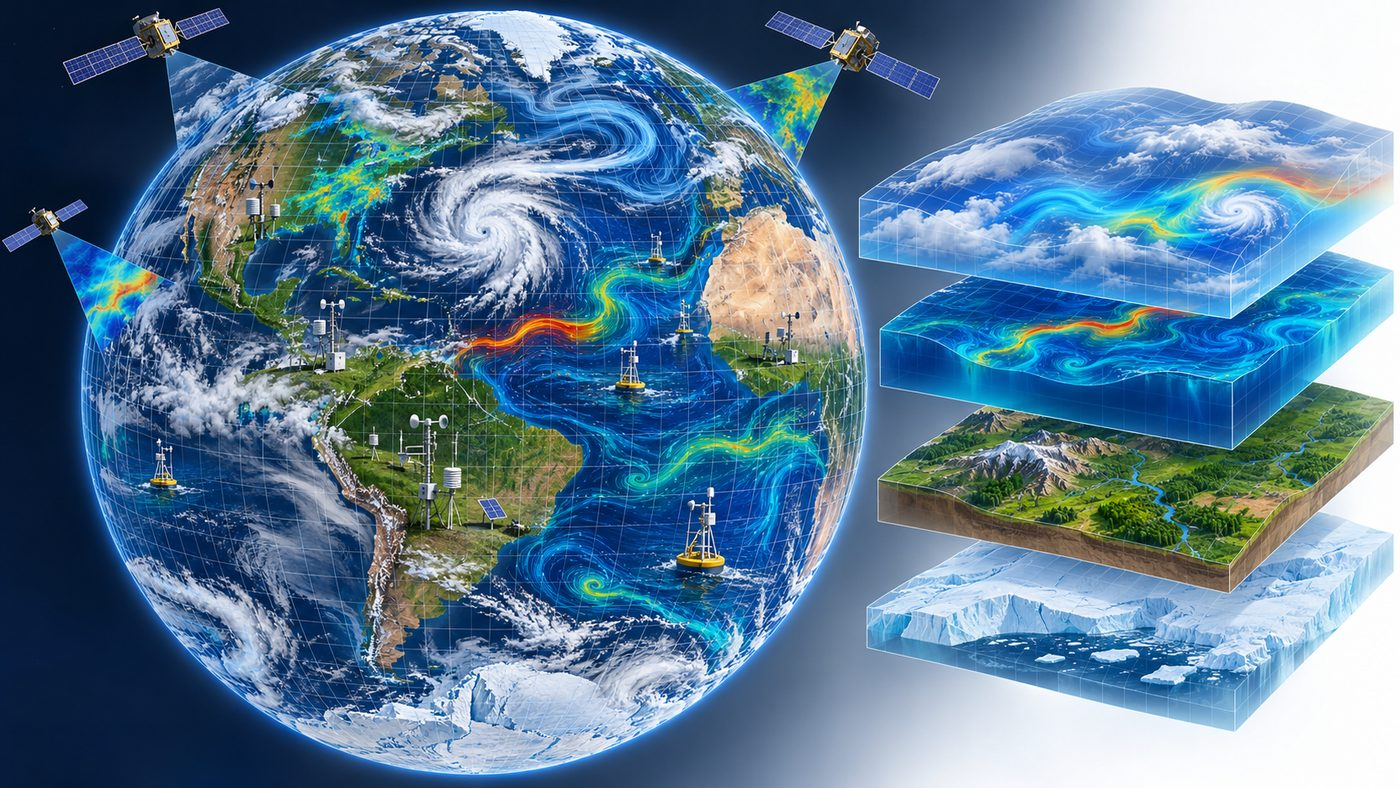
\includegraphics[width=\linewidth,height=5.25cm,keepaspectratio]{figures/climate_digital_twin.jpg}\\[-1mm]
\pdpsource{Ilustrasi konseptual Earth-system digital twin untuk pembelajaran.}
\end{columns}
\end{frame}

% 4 -----------------------------------------------------------------
\begin{frame}{Dari Transport Orde Satu ke Mekanisme PDP Orde Dua}
\footnotesize
\begin{columns}[T,onlytextwidth]
\column{0.41\textwidth}
\centering
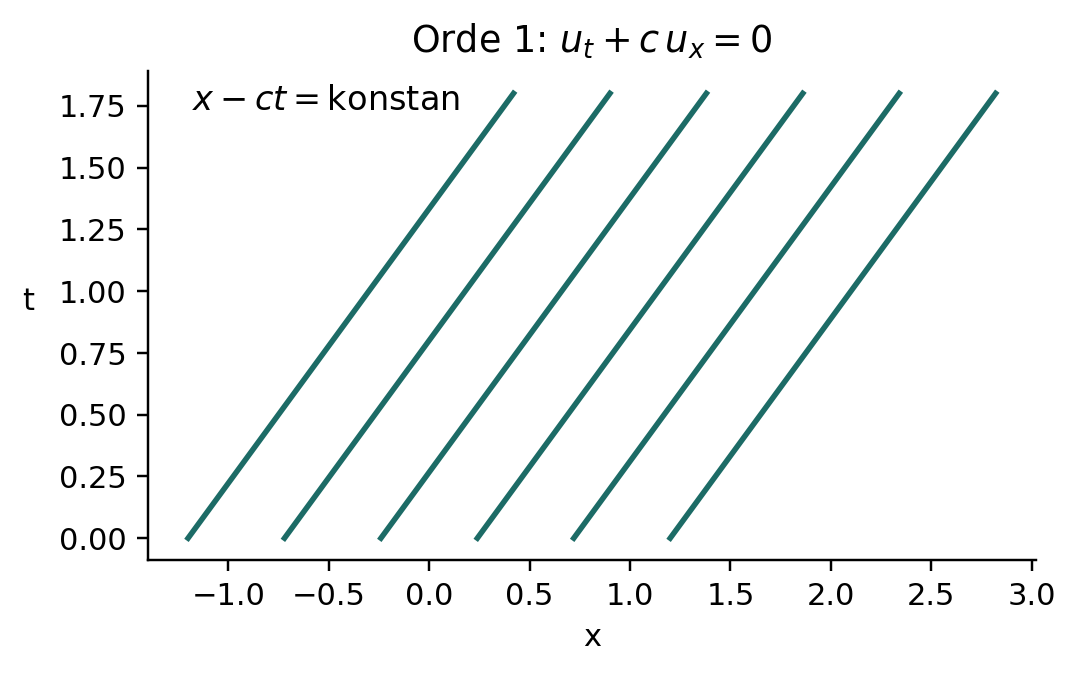
\includegraphics[width=.95\linewidth,height=3.4cm,keepaspectratio]{figures/transport_characteristics.png}

\vspace{0.08cm}
\small
Untuk
\[
 u_t+c u_x=0,
\]
nilai dibawa sepanjang
\[
 x-ct=\text{konstan}.
\]
Karakteristik memberi cara geometris untuk membaca \textbf{transfer informasi}.

\column{0.56\textwidth}
\small
Pada PDP orde dua, struktur turunan tertinggi membedakan mekanisme yang berbeda.

\vspace{0.10cm}
\begin{tabular}{@{}>{\raggedright\arraybackslash}p{1.85cm} >{\raggedright\arraybackslash}p{4.75cm}@{}}
\toprule
\textbf{Mekanisme} & \textbf{Perilaku utama}\\
\midrule
Kesetimbangan & medan ditentukan oleh kondisi pada batas domain; tidak ada arah rambat waktu intrinsik.\\[3pt]
Difusi & profil berubah terhadap waktu dan cenderung dihaluskan.\\[3pt]
Gelombang & gangguan merambat dengan kecepatan hingga; informasi memiliki domain pengaruh.\\
\bottomrule
\end{tabular}
\end{columns}
\end{frame}

% 5 -----------------------------------------------------------------
\begin{frame}{Banyak Sistem Nyata Digovern oleh Persamaan Diferensial}
\begin{columns}[T,onlytextwidth]
\column{0.49\textwidth}
\centering
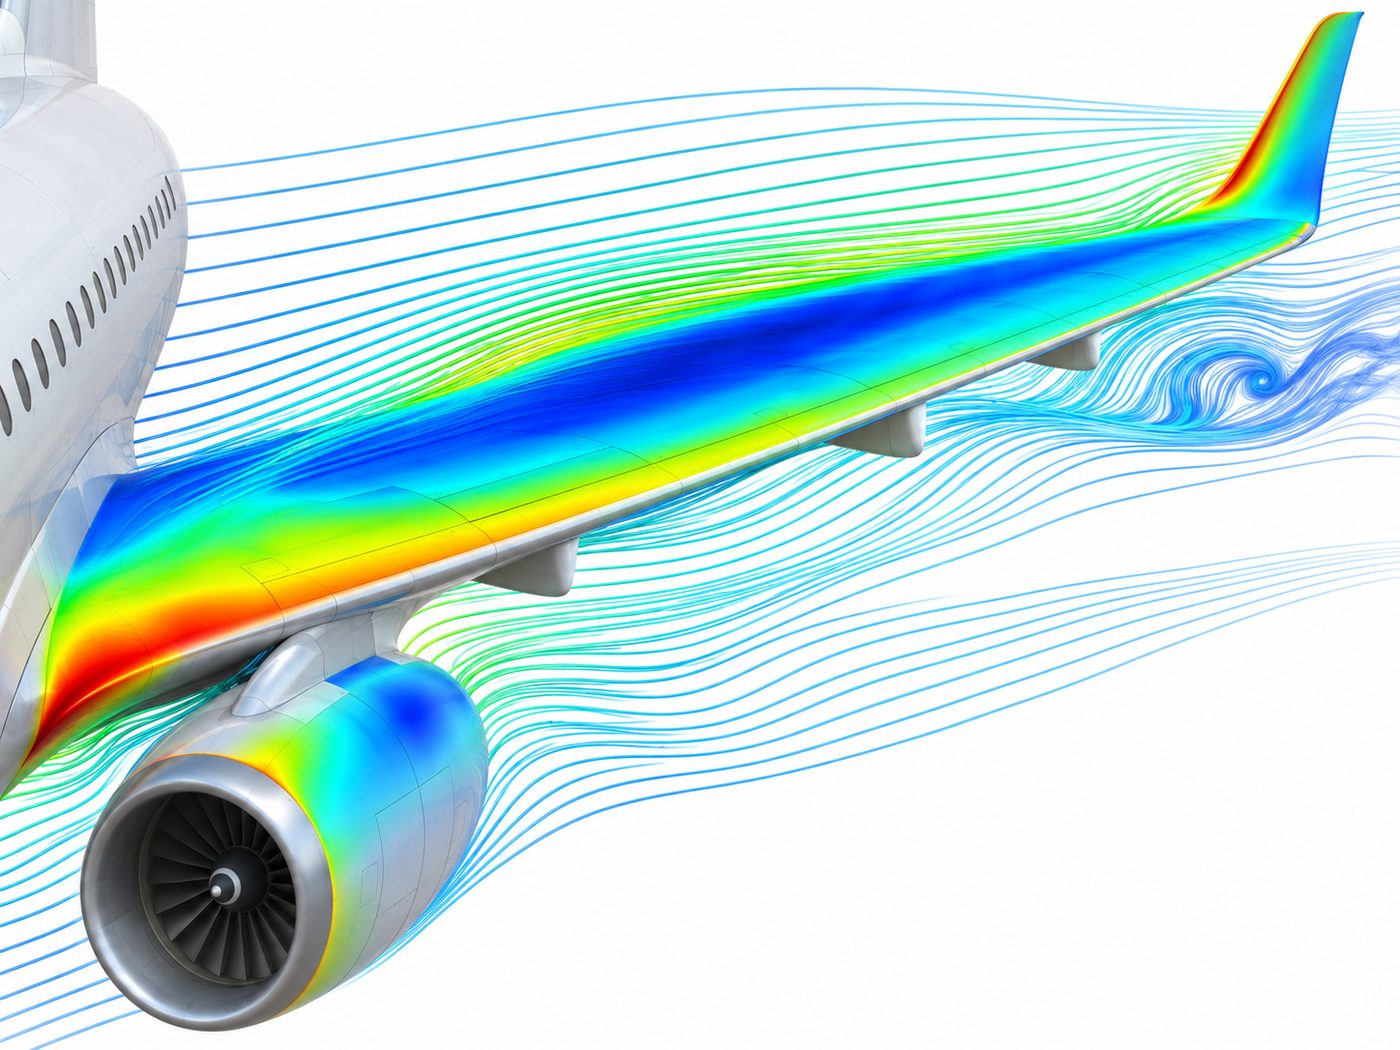
\includegraphics[width=.93\linewidth,height=2.18cm,keepaspectratio]{figures/aircraft_cfd.jpg}\\[-1mm]
{\scriptsize Aerodinamika: Navier--Stokes, akustik, elastodinamika.}

\vspace{0.16cm}
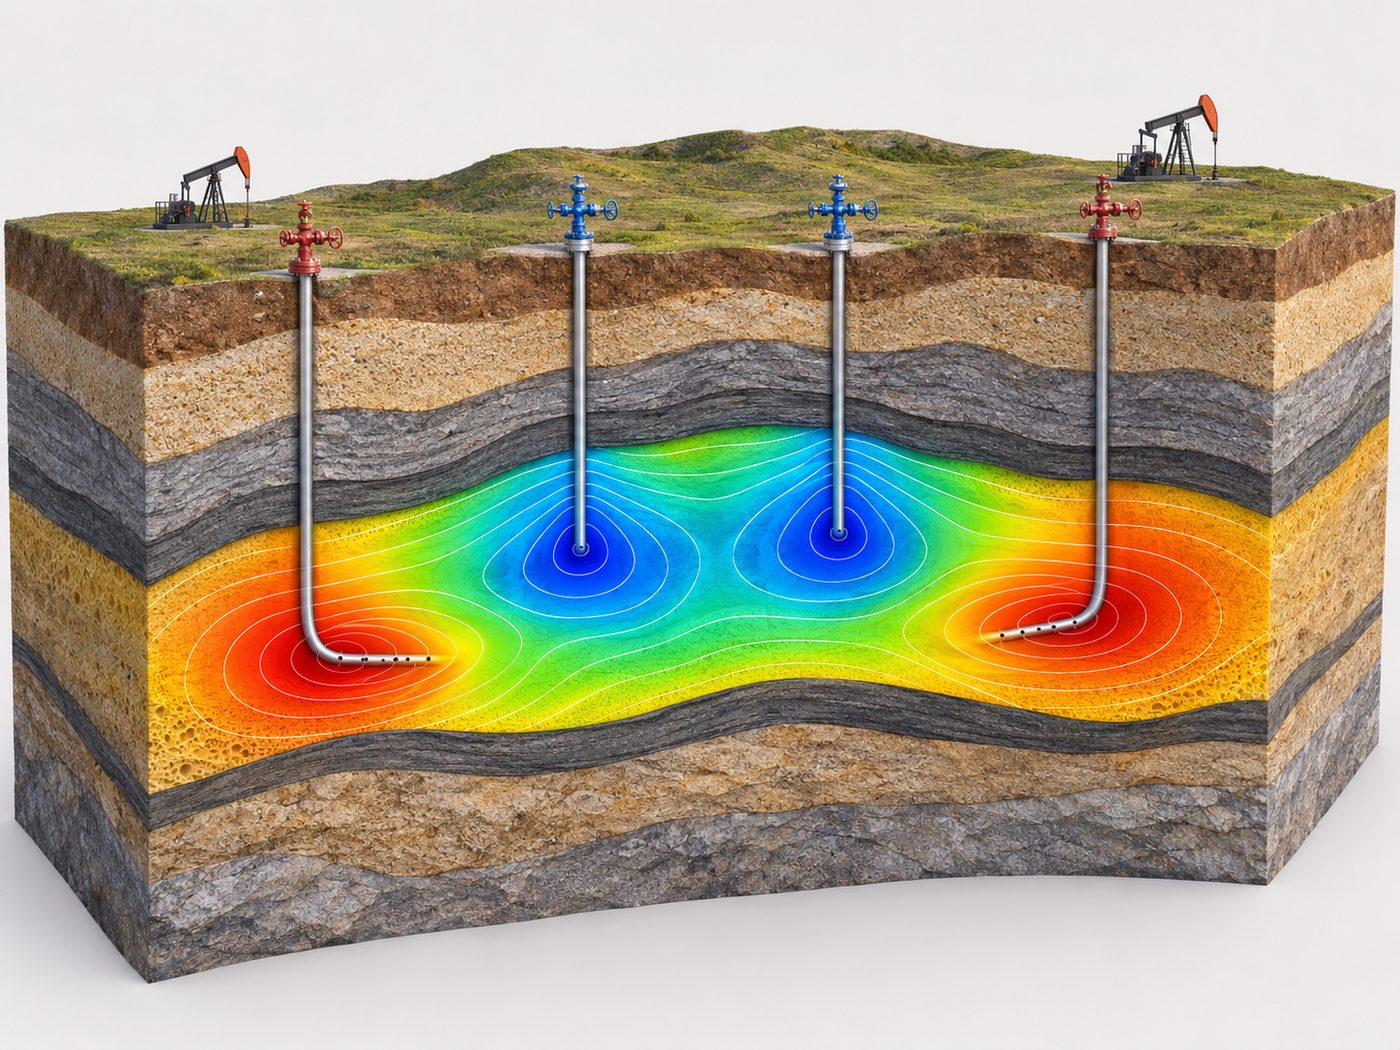
\includegraphics[width=.93\linewidth,height=2.18cm,keepaspectratio]{figures/reservoir.jpg}\\[-1mm]
{\scriptsize Reservoir: tekanan, aliran berpori, transport fluida.}

\column{0.49\textwidth}
\centering
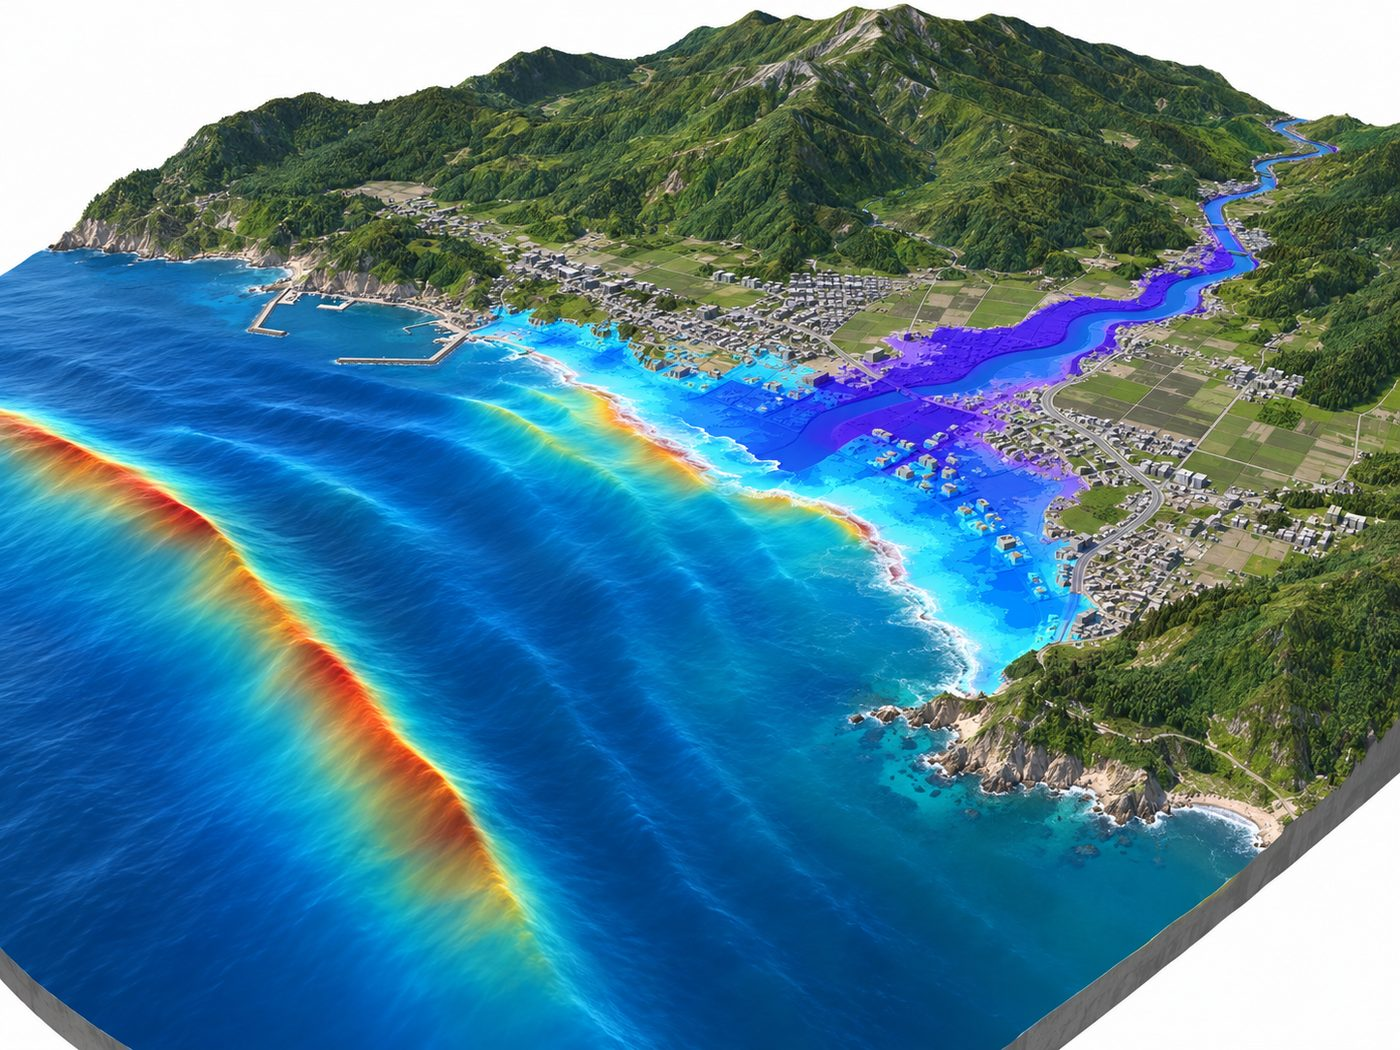
\includegraphics[width=.93\linewidth,height=2.18cm,keepaspectratio]{figures/coastal_hazard.jpg}\\[-1mm]
{\scriptsize Pesisir: shallow-water, tsunami, banjir, inundasi.}

\vspace{0.16cm}
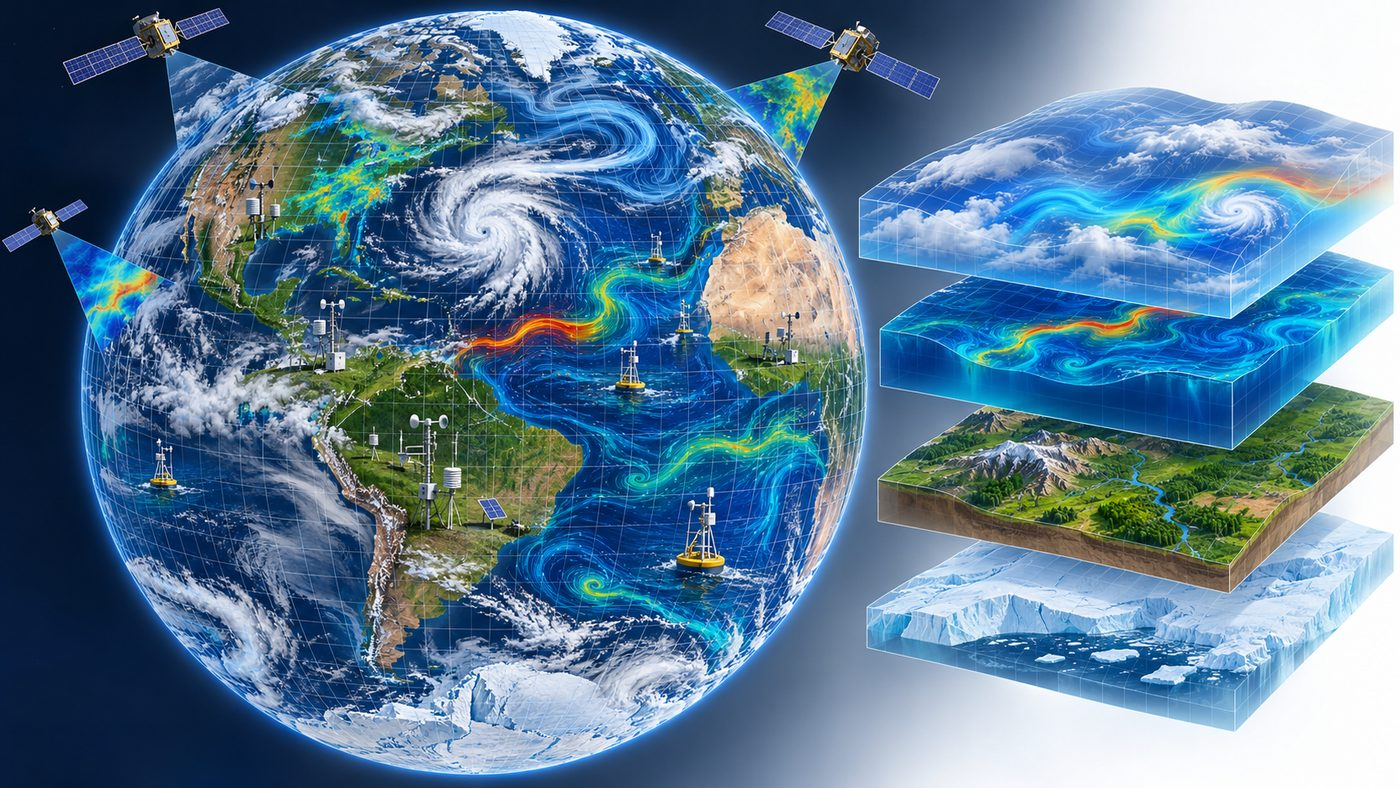
\includegraphics[width=.93\linewidth,height=2.18cm,keepaspectratio]{figures/climate_digital_twin.jpg}\\[-1mm]
{\scriptsize Iklim: atmosfer--laut--darat--es dan banyak skala ruang--waktu.}
\end{columns}
\end{frame}

% 6 -----------------------------------------------------------------
\begin{frame}{Mengapa Simulasi Numerik Menjadi Diperlukan?}
\begin{columns}[T,onlytextwidth]
\column{0.47\textwidth}
\begin{block}{Pada model ideal}
\begin{itemize}
  \item geometri sederhana;
  \item koefisien konstan;
  \item syarat batas teratur;
  \item forcing sederhana;
  \item solusi dapat diperoleh dalam bentuk tertutup atau deret.
\end{itemize}
\end{block}
\column{0.49\textwidth}
\begin{block}{Pada masalah nyata}
\begin{itemize}
  \item bentuk sayap, pantai, struktur, atau reservoir kompleks;
  \item material dan parameter heterogen;
  \item forcing tidak periodik dan data tidak sempurna;
  \item sistem nonlinear dan terkopel;
  \item banyak skala ruang dan waktu.
\end{itemize}
\end{block}
\end{columns}
\vspace{0.14cm}
\begin{beamercolorbox}[sep=.10cm,wd=\textwidth]{normal text}
\centering\small
Solusi analitik tetap penting sebagai \textbf{pemahaman dan benchmark}. Simulasi numerik memperluas model ke kondisi yang tidak lagi mudah diselesaikan secara analitik.
\end{beamercolorbox}
\end{frame}

% 7 -----------------------------------------------------------------
\begin{frame}{Contoh Governing PDE yang Digunakan dalam Aplikasi}
\scriptsize
\renewcommand{\arraystretch}{1.18}
\begin{tabular}{@{}>{\raggedright\arraybackslash}p{2.55cm} >{\raggedright\arraybackslash}p{6.3cm} >{\raggedright\arraybackslash}p{3.4cm}@{}}
\toprule
\textbf{Bidang / model} & \textbf{Bentuk yang muncul} & \textbf{Struktur}\\
\midrule
Aerodinamika, mesin & $\rho(\mathbf u_t+\mathbf u\cdot\nabla\mathbf u)=-\nabla p+\mu\nabla^2\mathbf u+\mathbf f$ & propagasi, difusi, constraint; tipe bergantung regime\\[3pt]
Laut, tsunami, banjir & $h_t+(hu)_x=0$, $u_t+u u_x+g h_x=0$ & sistem nonlinear hiperbolik (inviscid, 1D)\\[3pt]
Reservoir & $\phi c_t p_t-\nabla\cdot((k/\mu)\nabla p)=q$ & parabolik; steady-state menjadi eliptik\\[3pt]
Keuangan & $V_t+\tfrac12\sigma^2S^2V_{SS}+rSV_S-rV=0$ & parabolik (Black--Scholes)\\[3pt]
Struktur & $\rho u_{tt}-\nabla\cdot\sigma(u)=f$ & dinamika elastik: hiperbolik\\
\bottomrule
\end{tabular}
\vspace{0.12cm}
\par\pdpnote{Nama bidang tidak menentukan satu tipe PDP. Tipe ditentukan oleh principal part dan regime/model yang sedang dianalisis.}
\end{frame}

% 8 -----------------------------------------------------------------
\begin{frame}{Tiga Pertanyaan yang Harus Dibedakan}
\begin{columns}[T,onlytextwidth]
\column{0.31\textwidth}
\begin{block}{Linear atau nonlinear?}
Apakah $u$ dan turunannya muncul secara linear?

\vspace{0.12cm}
Contoh nonlinear:
\[
 u_t+u u_x=0.
\]
\end{block}
\column{0.31\textwidth}
\begin{block}{Homogen atau nonhomogen?}
Apakah ada forcing/sumber yang tidak nol?

\vspace{0.12cm}
Contoh:
\[
 u_{tt}-c^2u_{xx}=f(x,t).
\]
\end{block}
\column{0.31\textwidth}
\begin{block}{Eliptik, parabolik, hiperbolik?}
Ditentukan oleh \textbf{principal part}, yaitu struktur turunan orde tertinggi.

\vspace{0.12cm}
Ini adalah klasifikasi yang berbeda dari linearitas dan kehomogenan.
\end{block}
\end{columns}
\end{frame}

% 9 -----------------------------------------------------------------
\begin{frame}{Klasifikasi PDP Orde Dua dari Principal Part}
\small
Untuk dua variabel $x,y$, tuliskan
\[
A u_{xx}+2B u_{xy}+C u_{yy}+D u_x+E u_y+Fu=G.
\]
Principal part adalah
\[
L_2u=A u_{xx}+2B u_{xy}+C u_{yy}.
\]
Definisikan
\[
\Delta=B^2-AC.
\]
\vspace{0.05cm}
\renewcommand{\arraystretch}{1.18}
\begin{tabular}{@{}>{\raggedright\arraybackslash}p{2.1cm} >{\centering\arraybackslash}p{2.0cm} >{\raggedright\arraybackslash}p{6.8cm}@{}}
\toprule
\textbf{Tipe} & \textbf{Tanda $\Delta$} & \textbf{Interpretasi lokal}\\
\midrule
Eliptik & $<0$ & tidak terdapat arah karakteristik real.\\[2pt]
Parabolik & $=0$ & terdapat satu arah karakteristik real yang berulang.\\[2pt]
Hiperbolik & $>0$ & terdapat dua arah karakteristik real.\\
\bottomrule
\end{tabular}
\vspace{0.10cm}
\pdpnote{Jika buku menulis suku silang sebagai $B u_{xy}$, diskriminan yang digunakan menjadi $B^2-4AC$.}
\end{frame}

% 10 ----------------------------------------------------------------
\begin{frame}{Mengapa Namanya Eliptik, Parabolik, dan Hiperbolik?}
\begin{columns}[T,onlytextwidth]
\column{0.48\textwidth}
\small
Bentuk kuadratik
\[
Ax^2+2Bxy+Cy^2+Dx+Ey+F=0
\]
mempunyai diskriminan yang sama,
\[
\Delta=B^2-AC.
\]
Setelah rotasi/translasi koordinat, tanda $\Delta$ membedakan ellipse, parabola, dan hyperbola.

\vspace{0.15cm}
\begin{block}{Tetapi hati-hati}
Nama tersebut tidak berarti grafik solusi $u(x,y)$ berbentuk ellipse, parabola, atau hyperbola. Hubungan geometris yang relevan untuk PDP muncul melalui \textbf{arah karakteristik}.
\end{block}
\column{0.50\textwidth}
\centering
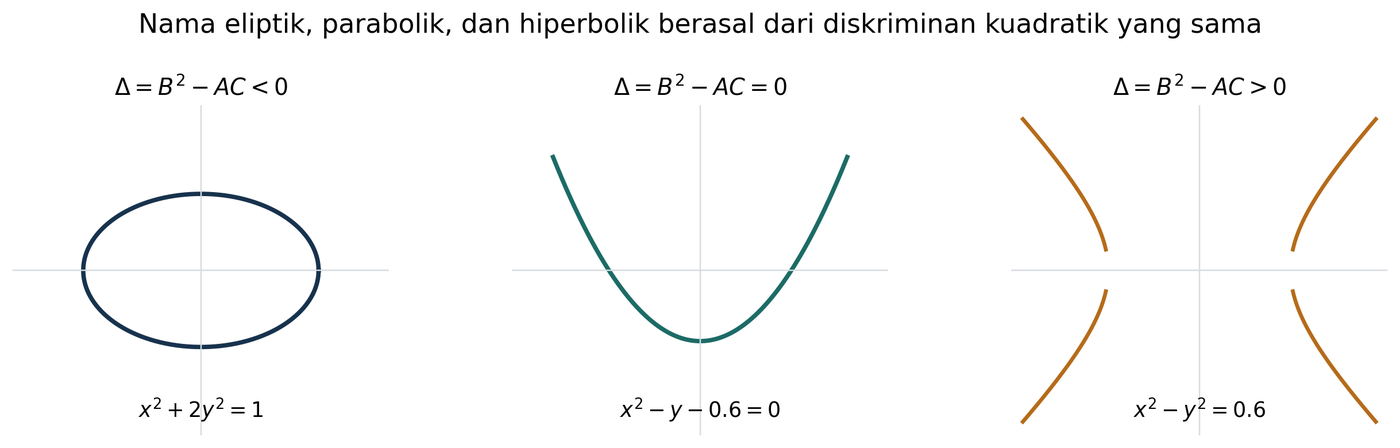
\includegraphics[width=.98\linewidth,height=4.65cm,keepaspectratio]{figures/conic_discriminant.png}
\end{columns}
\end{frame}

% 11 ----------------------------------------------------------------
\begin{frame}{Dari $u_{xx}$ ke $(dy)^2$: Asal Persamaan Karakteristik}
\small
Ambil koordinat baru $\xi=\phi(x,y)$ dan $\eta=\psi(x,y)$, dengan $u(x,y)=U(\xi,\eta)$. Aturan rantai memberi, pada bagian orde dua,
\[
 u_{xx}=U_{\xi\xi}\phi_x^2+2U_{\xi\eta}\phi_x\psi_x+U_{\eta\eta}\psi_x^2+\cdots
\]
serta bentuk serupa untuk $u_{xy}$ dan $u_{yy}$.

Koefisien $U_{\xi\xi}$ dalam principal part adalah
\[
 A\phi_x^2+2B\phi_x\phi_y+C\phi_y^2.
\]
Pada kurva level $\phi(x,y)=\text{konstan}$ berlaku
\[
 d\phi=\phi_x\,dx+\phi_y\,dy=0.
\]
Karena $(\phi_x,\phi_y)$ tegak lurus arah tangent $(dx,dy)$, secara proporsional dapat diambil $\phi_x\sim dy$, $\phi_y\sim-dx$. Maka
\[
\boxed{A(dy)^2-2B\,dx\,dy+C(dx)^2=0.}
\]
\pdpnote{$u_{xx}$ tidak ``berubah menjadi'' $dy^2$; persamaan kuadratik ini muncul saat kita mencari arah koordinat yang menghilangkan salah satu turunan orde dua.}
\end{frame}

% 12 ----------------------------------------------------------------
\begin{frame}{Prosedur Memeriksa Klasifikasi dan Bentuk Kanonik}
\begin{columns}[T,onlytextwidth]
\column{0.46\textwidth}
\begin{block}{Langkah pemeriksaan}
\begin{enumerate}
  \item Identifikasi variabel bebas.
  \item Ambil hanya principal part.
  \item Baca $A$, $B$, $C$ dari $A u_{xx}+2B u_{xy}+C u_{yy}$.
  \item Hitung $\Delta=B^2-AC$.
  \item Cari kurva karakteristik jika $\Delta\ge0$.
  \item Pilih koordinat karakteristik / rotasi yang menyederhanakan principal part.
\end{enumerate}
\end{block}
\column{0.50\textwidth}
\begin{block}{Bentuk kanonik lokal}
Setelah perubahan koordinat dan skala yang sesuai:
\[
\begin{array}{ll}
\text{eliptik:} & U_{\xi\xi}+U_{\eta\eta}+\text{orde rendah}=\widetilde G,\\[3pt]
\text{parabolik:} & U_{\xi\xi}+\text{orde rendah}=\widetilde G,\\[3pt]
\text{hiperbolik:} & U_{\xi\eta}+\text{orde rendah}=\widetilde G.
\end{array}
\]
\end{block}
\end{columns}
\end{frame}

% 13 ----------------------------------------------------------------
\begin{frame}{Model Fisis: Dawai yang Bergetar}
\begin{columns}[T,onlytextwidth]
\column{0.49\textwidth}
\centering
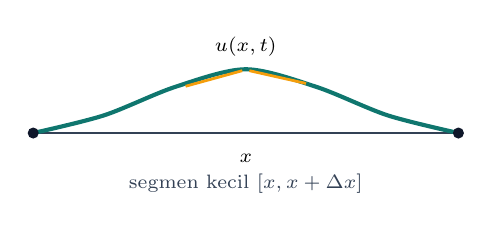
\begin{tikzpicture}[x=.9cm,y=.9cm]
\draw[pdpSlate,line width=1.0pt] (0,0)--(6,0);
\draw[pdpTeal,line width=1.5pt] plot[smooth] coordinates {(0,0)(1,.25)(2,.65)(3,.9)(4,.65)(5,.25)(6,0)};
\fill[pdpNavy] (0,0) circle (2pt); \fill[pdpNavy] (6,0) circle (2pt);
\draw[pdpAmber,line width=1pt] (2.15,.66)--(2.95,.88);
\draw[pdpAmber,line width=1pt] (3.05,.88)--(3.85,.70);
\node[font=\scriptsize] at (3,-.35) {$x$};
\node[font=\scriptsize] at (3,1.22) {$u(x,t)$};
\node[font=\scriptsize,text=pdpSlate] at (3,-.72) {segmen kecil $[x,x+\Delta x]$};
\end{tikzpicture}
\column{0.47\textwidth}
\begin{block}{Asumsi model linear}
\begin{itemize}
  \item Dawai homogen dengan rapat massa linear $\rho$ konstan.
  \item Tegangan $T$ dianggap konstan.
  \item Gerak hanya transversal; perpindahan longitudinal diabaikan.
  \item Dawai fleksibel; kekakuan lentur diabaikan.
  \item Kemiringan kecil: $|u_x|\ll1$.
  \item Tidak ada redaman dan gaya luar pada model dasar.
\end{itemize}
\end{block}
\end{columns}
\vspace{0.10cm}
\pdpnote{Asumsi kecil-slope adalah kunci linearitas. Jika deformasi besar atau tegangan berubah, model gelombang linear tidak lagi memadai.}
\end{frame}

% 14 ----------------------------------------------------------------
\begin{frame}{Penurunan Persamaan Gelombang dari Neraca Gaya}
\small
Ambil segmen $[x,x+\Delta x]$. Komponen vertikal gaya tegangan adalah
\[
T\sin\theta(x+\Delta x,t)-T\sin\theta(x,t).
\]
Untuk kemiringan kecil,
\[
\sin\theta\approx\tan\theta=u_x.
\]
Maka resultan gaya vertikal
\[
T\bigl[u_x(x+\Delta x,t)-u_x(x,t)\bigr]
\approx T u_{xx}(x,t)\,\Delta x.
\]
Massa segmen adalah $\rho\Delta x$. Hukum II Newton memberi
\[
\rho\Delta x\,u_{tt}=T u_{xx}\Delta x.
\]
Setelah membagi dengan $\rho\Delta x$,
\[
\boxed{u_{tt}=c^2u_{xx}},\qquad \boxed{c=\sqrt{\frac{T}{\rho}}}.
\]
\pdpnote{$c$ adalah kecepatan rambat gangguan pada model dawai linear.}
\end{frame}

% 15 ----------------------------------------------------------------
\begin{frame}{Klasifikasi Persamaan Gelombang}
\begin{columns}[T,onlytextwidth]
\column{0.47\textwidth}
\small
Gunakan variabel $(x,t)$:
\[
 u_{tt}-c^2u_{xx}=0.
\]
Dalam bentuk
\[
A u_{xx}+2B u_{xt}+C u_{tt}=0
\]
diperoleh
\[
A=-c^2,\qquad B=0,\qquad C=1.
\]
Sehingga
\[
\Delta=B^2-AC=c^2>0.
\]
\begin{block}{Kesimpulan}
Persamaan gelombang adalah \textbf{hiperbolik}.
\end{block}
\column{0.49\textwidth}
\centering
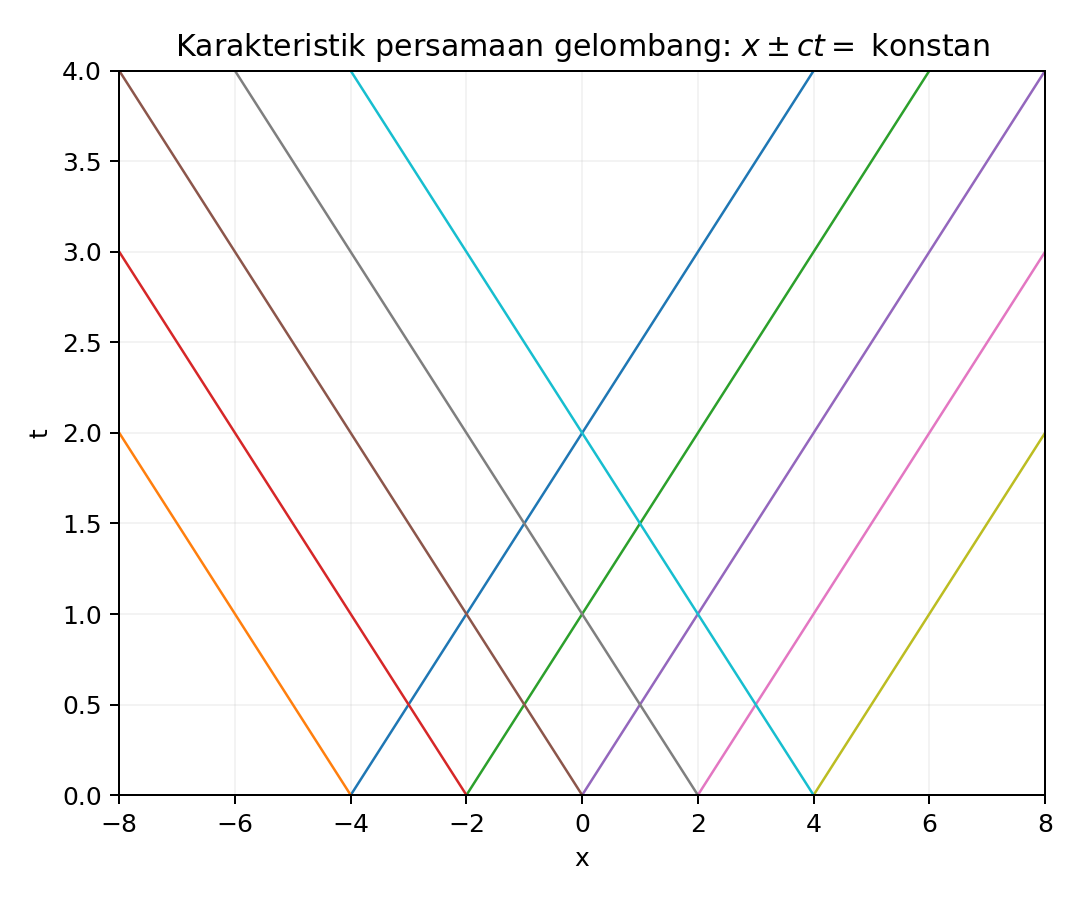
\includegraphics[width=.90\linewidth,height=4.45cm,keepaspectratio]{figures/wave_characteristics.png}
\end{columns}
\end{frame}

% 16 ----------------------------------------------------------------
\begin{frame}{Karakteristik dan Bentuk Kanonik Persamaan Gelombang}
\small
Persamaan karakteristiknya
\[
-c^2(dt)^2+(dx)^2=0,
\]
sehingga
\[
\frac{dx}{dt}=\pm c,
\qquad
x-ct=\text{konstan},\quad x+ct=\text{konstan}.
\]
Ambil koordinat karakteristik
\[
\xi=x-ct,\qquad \eta=x+ct.
\]
Jika $u(x,t)=U(\xi,\eta)$, maka
\[
 u_{xx}=U_{\xi\xi}+2U_{\xi\eta}+U_{\eta\eta},
\]
\[
 u_{tt}=c^2\left(U_{\xi\xi}-2U_{\xi\eta}+U_{\eta\eta}\right).
\]
Jadi
\[
 u_{tt}-c^2u_{xx}=-4c^2U_{\xi\eta}=0,
\qquad
\boxed{U_{\xi\eta}=0.}
\]
Inilah bentuk kanonik hiperbolik untuk persamaan gelombang satu dimensi.
\end{frame}

% 17 ----------------------------------------------------------------
\begin{frame}{Solusi d'Alembert: Dua Keluarga Gelombang Menjalar}
\begin{columns}[T,onlytextwidth]
\column{0.51\textwidth}
\small
Dari
\[
U_{\xi\eta}=0
\]
diperoleh
\[
U(\xi,\eta)=F(\xi)+G(\eta).
\]
Kembali ke $(x,t)$:
\[
\boxed{u(x,t)=F(x-ct)+G(x+ct).}
\]

\begin{block}{Makna}
$F(x-ct)$ bergerak ke kanan dan $G(x+ct)$ bergerak ke kiri tanpa mengubah bentuk pada model ideal.
\end{block}
\column{0.45\textwidth}
\centering
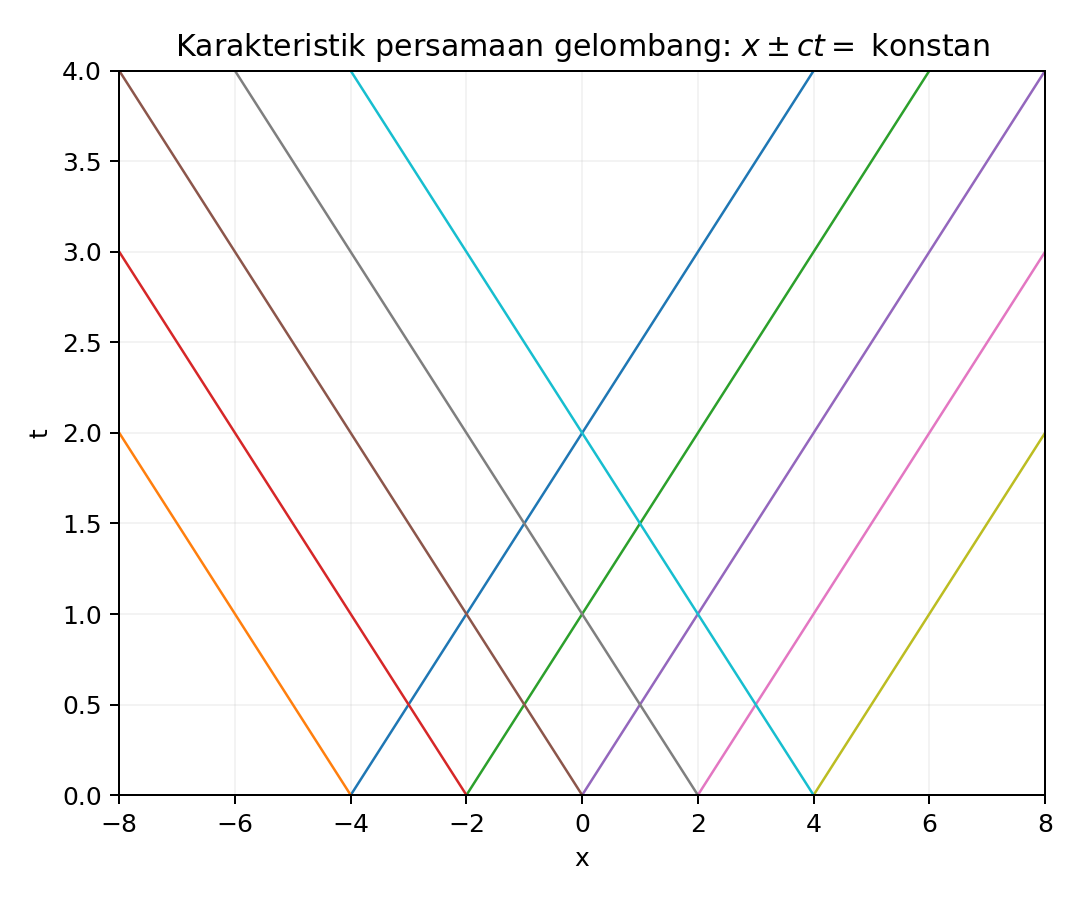
\includegraphics[width=.98\linewidth,height=4.45cm,keepaspectratio]{figures/wave_characteristics.png}
\end{columns}
\end{frame}

% 18 ----------------------------------------------------------------
\begin{frame}{Dawai dengan Kedua Ujung Terikat: Pemisahan Variabel}
\begin{columns}[T,onlytextwidth]
\column{0.50\textwidth}
\small
Untuk
\[
 u_{tt}=c^2u_{xx},\quad 0<x<L,
\]
dengan
\[
 u(0,t)=u(L,t)=0,
\]
ambil
\[
 u(x,t)=X(x)T(t).
\]
Substitusi memberi
\[
\frac{X''}{X}=\frac{T''}{c^2T}=-\lambda.
\]
Maka
\[
X''+\lambda X=0,
\qquad
T''+c^2\lambda T=0.
\]
\column{0.46\textwidth}
\begin{block}{Masalah nilai eigen}
Syarat $X(0)=X(L)=0$ menghasilkan
\[
\lambda_n=\left(\frac{n\pi}{L}\right)^2,
\qquad
X_n(x)=\sin\left(\frac{n\pi x}{L}\right).
\]
\end{block}
\begin{block}{Frekuensi alami}
\[
\omega_n=c\sqrt{\lambda_n}=\frac{n\pi c}{L}.
\]
Mode yang diizinkan ditentukan oleh geometri domain dan syarat batas.
\end{block}
\end{columns}
\end{frame}

% 19 ----------------------------------------------------------------
\begin{frame}{Solusi Umum untuk Dawai Terikat}
\small
Dengan kondisi awal
\[
 u(x,0)=f(x),\qquad u_t(x,0)=g(x),
\]
solusinya
\[
\boxed{
 u(x,t)=\sum_{n=1}^{\infty}
 \left[A_n\cos(\omega_n t)+B_n\sin(\omega_n t)\right]
 \sin\left(\frac{n\pi x}{L}\right)
}
\]
dengan
\[
A_n=\frac{2}{L}\int_0^L f(x)\sin\left(\frac{n\pi x}{L}\right)dx,
\]
\[
B_n=\frac{2}{n\pi c}\int_0^L g(x)\sin\left(\frac{n\pi x}{L}\right)dx.
\]
\begin{beamercolorbox}[sep=.10cm,wd=\textwidth]{normal text}
\centering\small
Deret Fourier bukan tambahan terpisah: ia menentukan seberapa besar setiap \textbf{mode eigen} hadir dalam kondisi awal.
\end{beamercolorbox}
\end{frame}

% 20 ----------------------------------------------------------------
\begin{frame}{Contoh Numerik-Analitik: Satu Mode Dawai}
\begin{columns}[T,onlytextwidth]
\column{0.39\textwidth}
\small
Ambil
\[
L=10\text{ m},\qquad c=2\text{ m/s},
\]
\[
f(x)=0.1\sin\left(\frac{\pi x}{10}\right),\qquad g(x)=0.
\]
Hanya mode $n=1$ yang aktif:
\[
\boxed{
 u(x,t)=0.1\sin\left(\frac{\pi x}{10}\right)
 \cos\left(\frac{\pi t}{5}\right)}.
\]
Periode osilasi:
\[
T_1=\frac{2\pi}{\omega_1}=10\text{ s}.
\]
\column{0.58\textwidth}
\centering
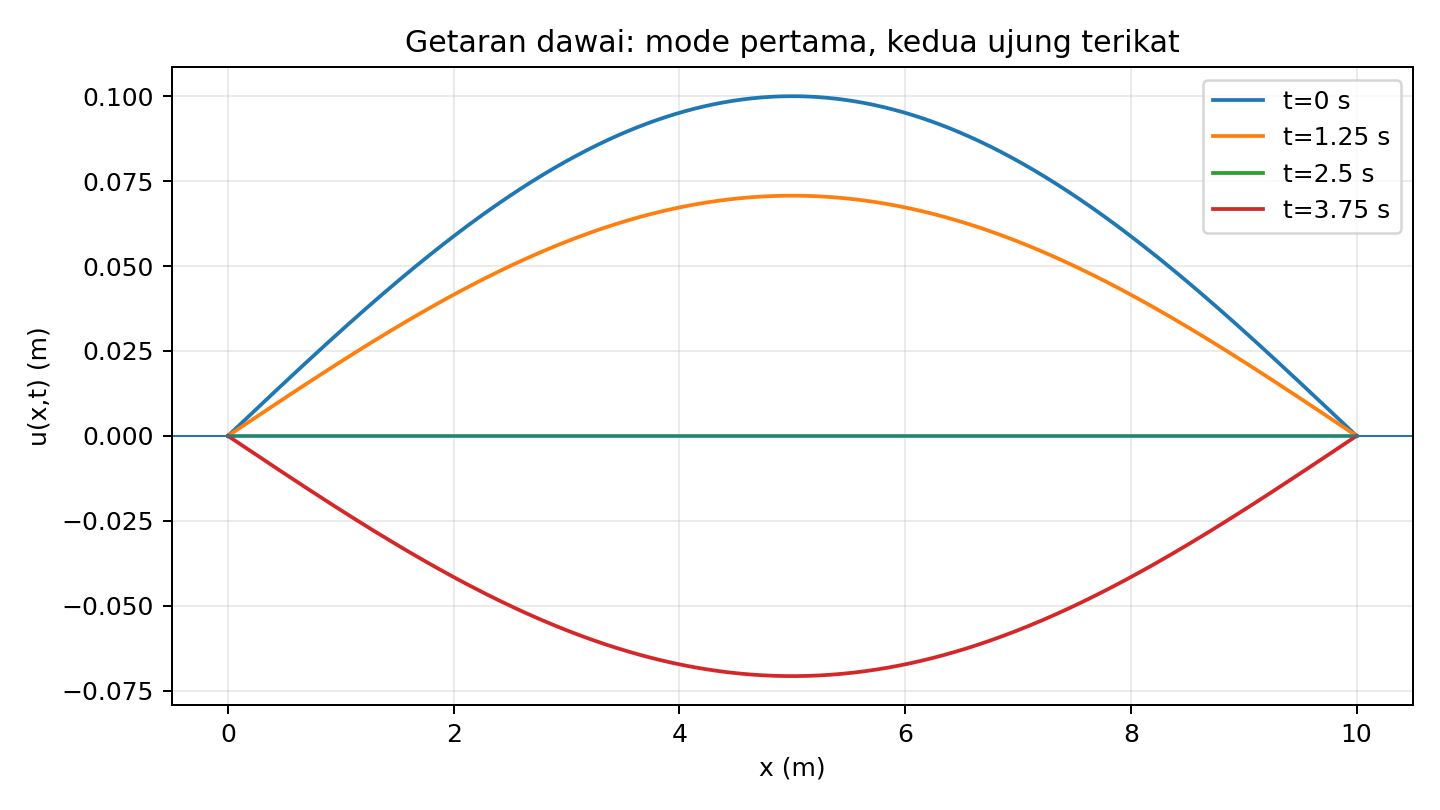
\includegraphics[width=\linewidth,height=4.7cm,keepaspectratio]{figures/string_mode1.png}
\end{columns}
\end{frame}

% 21 ----------------------------------------------------------------
\begin{frame}{Dari Shallow-Water Nonlinear ke Persamaan Gelombang}
\begin{columns}[T,onlytextwidth]
\column{0.51\textwidth}
\small
Untuk aliran 1D, dasar datar, inviscid, dan tekanan hidrostatik, shallow-water dapat ditulis
\[
 h_t+(hu)_x=0,
\]
\[
 u_t+u u_x+g h_x=0.
\]
Tuliskan
\[
 h(x,t)=H+\eta(x,t),
\]
dengan $H$ kedalaman rata-rata dan $\eta$ deviasi muka air.

\column{0.45\textwidth}
\begin{block}{Asumsi linearisasi}
\begin{itemize}
  \item $|\eta|/H\ll1$;
  \item kecepatan $u$ kecil terhadap skala gelombang;
  \item produk gangguan kecil $(\eta u)_x$ diabaikan;
  \item nonlinearitas advektif $u u_x$ diabaikan;
  \item $H$ konstan, dasar datar.
\end{itemize}
\end{block}
\end{columns}
\vspace{0.10cm}
Setelah linearisasi:
\[
\boxed{\eta_t+H u_x=0},\qquad
\boxed{u_t+g\eta_x=0}.
\]
\end{frame}

% 22 ----------------------------------------------------------------
\begin{frame}{Persamaan Gelombang Air Dangkal Linear}
\begin{columns}[T,onlytextwidth]
\column{0.45\textwidth}
\small
Diferensiasikan kontinuitas terhadap $t$:
\[
\eta_{tt}+H u_{xt}=0.
\]
Dari persamaan momentum,
\[
u_t=-g\eta_x
\quad\Rightarrow\quad
u_{xt}=-g\eta_{xx}.
\]
Maka
\[
\boxed{\eta_{tt}-gH\eta_{xx}=0},
\qquad
\boxed{c=\sqrt{gH}}.
\]
Solusi analitik umum:
\[
\boxed{\eta=F(x-ct)+G(x+ct)}.
\]
\column{0.52\textwidth}
\centering
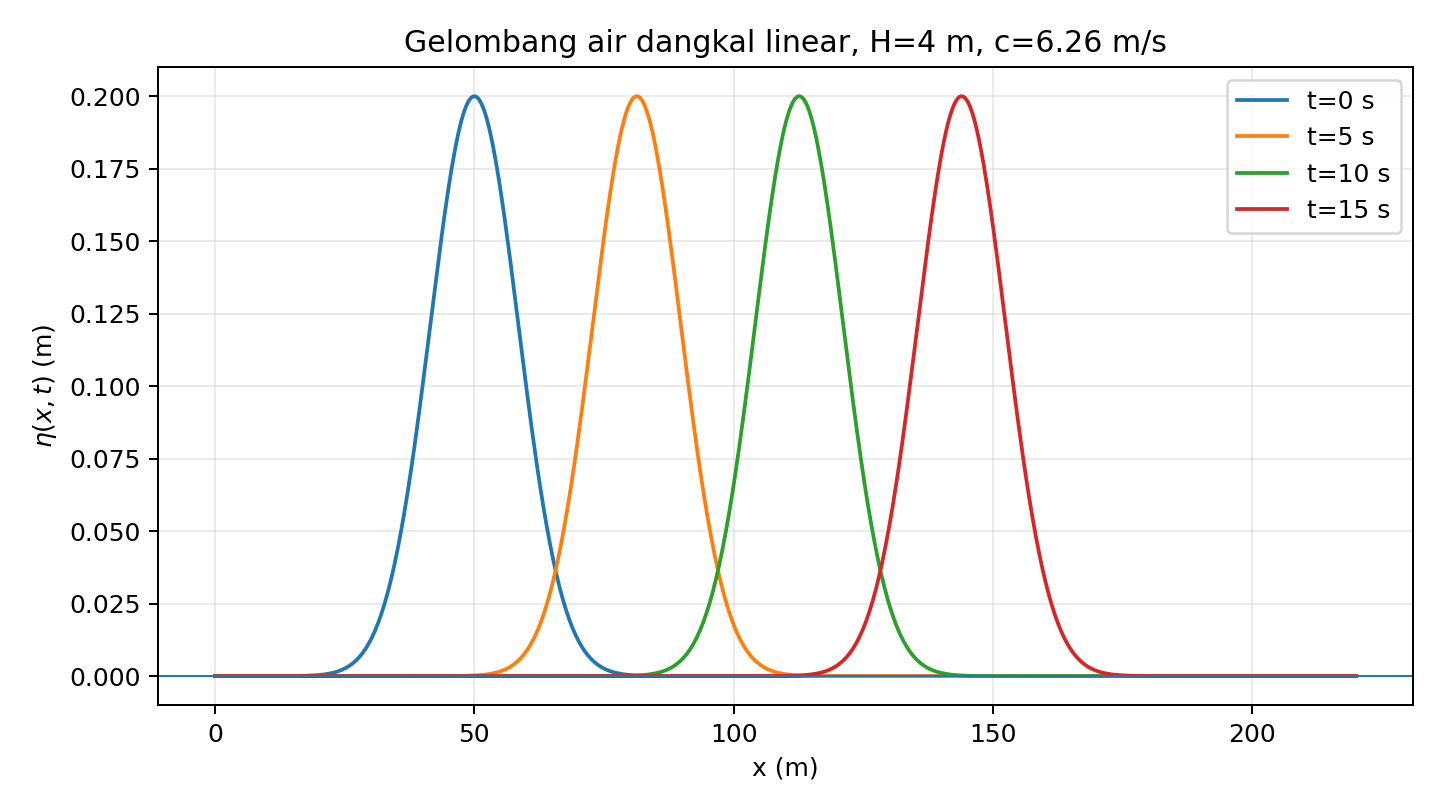
\includegraphics[width=\linewidth,height=4.65cm,keepaspectratio]{figures/shallow_water_gaussian.png}
\end{columns}
\end{frame}

% 23 ----------------------------------------------------------------
\begin{frame}{Interpretasi Solusi Shallow-Water Linear}
\small
Jika kondisi awal adalah elevasi $\eta(x,0)=f(x)$ dan kecepatan awal nol, maka
\[
\boxed{\eta(x,t)=\frac12f(x-ct)+\frac12f(x+ct)}.
\]
Pulsa awal terpecah menjadi dua gelombang dengan amplitudo setengah yang bergerak berlawanan arah.

\vspace{0.20cm}
Untuk satu gelombang yang hanya bergerak ke kanan, kondisi awal kecepatan harus kompatibel:
\[
\eta(x,t)=f(x-ct),
\qquad
u(x,t)=\frac{c}{H}f(x-ct)=\sqrt{\frac{g}{H}}f(x-ct).
\]
\begin{block}{Makna pemodelan}
Persamaan gelombang klasik muncul sebagai \textbf{aproksimasi linear} dari sistem shallow-water nonlinear. Karena itu, sebelum memakai solusi analitik gelombang, kita harus mengetahui asumsi yang membuat linearisasi tersebut sah.
\end{block}
\end{frame}

% 24 ----------------------------------------------------------------
\begin{frame}{Latihan Individu: Klasifikasi, Kanonik, dan Solusi Analitik}
\small
\textbf{Bagian A - karakteristik dan bentuk kanonik}
\[
\boxed{u_{xx}+4u_{xt}+3u_{tt}=0.}
\]
\begin{enumerate}
  \item Tentukan $A,B,C$ dan klasifikasikan PDP.
  \item Tentukan dua keluarga kurva karakteristik.
  \item Pilih koordinat kanonik dan ubah PDP ke bentuk kanonik.
  \item Tuliskan bentuk umum solusi analitiknya.
\end{enumerate}

\vspace{0.16cm}
\textbf{Bagian B - vibrating string dengan angka}
\[
 u_{tt}-4u_{xx}=0,\quad 0<x<6,
\]
\[
 u(0,t)=u(6,t)=0,
\]
\[
 u(x,0)=0.12\sin\frac{\pi x}{6}+0.05\sin\frac{\pi x}{3},
\qquad u_t(x,0)=0.
\]
Tentukan solusi analitik dan gambarkan $u(x,t)$ untuk $t=0,1,2$ s.
\end{frame}

% 25 ----------------------------------------------------------------
\begin{frame}{Latihan Lanjutan: Kasus Nonhomogen}
\small
Sebagai pengayaan, pertimbangkan
\[
\boxed{u_{tt}-4u_{xx}=0.1\sin\left(\frac{\pi x}{6}\right)},
\quad 0<x<6,
\]
dengan
\[
 u(0,t)=u(6,t)=0,
\qquad
u(x,0)=0,
\qquad
u_t(x,0)=0.
\]

\begin{block}{Hint}
Karena forcing hanya berada pada mode pertama, coba
\[
 u(x,t)=a(t)\sin\left(\frac{\pi x}{6}\right).
\]
Substitusi ke PDP akan menghasilkan PDB
\[
 a''(t)+\left(\frac{\pi}{3}\right)^2a(t)=0.1.
\]
Gunakan kondisi awal $a(0)=a'(0)=0$.
\end{block}

Gambarkan solusi untuk sedikitnya tiga waktu dan jelaskan makna forcing terhadap amplitudo getaran.
\end{frame}

% 26 ----------------------------------------------------------------
\begin{frame}{Ketentuan Laporan Latihan}
\begin{columns}[T,onlytextwidth]
\column{0.49\textwidth}
\begin{block}{Format}
\begin{itemize}
  \item Dikerjakan \textbf{individu} dan \textbf{ditulis tangan}.
  \item Gunakan cover dengan identitas: nama, NIM, kelas, mata kuliah, dan judul latihan.
  \item Tuliskan prosedur klasifikasi, transformasi kanonik, dan langkah solusi analitik; jangan hanya menulis hasil akhir.
  \item Gunakan satuan jika variabel memiliki makna fisis.
\end{itemize}
\end{block}
\column{0.47\textwidth}
\begin{block}{Visualisasi}
\begin{itemize}
  \item Grafik boleh digambar manual dengan skala yang jelas.
  \item Grafik dari MATLAB boleh dicetak dan ditempel pada laporan.
  \item Setiap grafik harus diberi $t$, label sumbu, dan interpretasi singkat.
\end{itemize}
\end{block}
\begin{block}{Yang dinilai}
Ketepatan matematika, keterlacakan langkah, kualitas gambar, dan kemampuan menghubungkan solusi dengan perilaku gelombang.
\end{block}
\end{columns}
\end{frame}

% 27 ----------------------------------------------------------------
\begin{frame}{Ringkasan Pertemuan}
\small
\begin{columns}[T,onlytextwidth]
\column{0.31\textwidth}
\begin{block}{Model}
Persamaan gelombang diperoleh dari hukum fisika dan asumsi. Pada vibrating string, small-slope dan tension konstan menghasilkan model linear.
\end{block}
\column{0.31\textwidth}
\begin{block}{Struktur}
Diskriminan principal part menentukan tipe. Untuk persamaan gelombang terdapat dua keluarga karakteristik real dan bentuk kanonik $U_{\xi\eta}=0$.
\end{block}
\column{0.31\textwidth}
\begin{block}{Solusi}
D'Alembert menjelaskan gelombang menjalar; pemisahan variabel dan fungsi eigen menjelaskan mode pada domain terbatas. Shallow-water linear kembali menghasilkan persamaan gelombang.
\end{block}
\end{columns}
\vspace{0.18cm}
\centering
\pdpnote{Pertemuan berikutnya dapat memakai solusi analitik ini sebagai benchmark sebelum membangun metode numerik untuk PDP orde dua.}
\end{frame}

\end{document}
